\documentclass[xcolor=table,dvipsnames]{beamer}

\usepackage{setspace}
\usepackage{tikzsymbols}
\usepackage{breakcites}
\usepackage{subcaption}
\usepackage[normalem]{ulem}

\usetheme{Madrid}
\usecolortheme{default}

\graphicspath{{../..}}
\hbadness 10000
\vbadness 10000
\hfuzz 100pt
\vfuzz 100pt
\righthyphenmin 100

\setbeamertemplate{navigation symbols}{}
\setbeamertemplate{caption}[numbered]
\setbeamertemplate{itemize items}[circle]
\setbeamertemplate{enumerate items}[default]
\setbeamertemplate{section in toc}[circle]
\setbeamertemplate{title page}[default]

\setbeamerfont{itemize/enumerate body}{size=\normalsize}
\setbeamerfont{itemize/enumerate subbody}{size=\normalsize}
\setbeamerfont{title}{size=\Huge}
\setbeamerfont{subtitle}{size=\large}
\setbeamerfont{author}{size=\large}
\setbeamerfont{institute}{size=\large}
\setbeamerfont{date}{size=\large}

\title{Variational Autoencoders}
\subtitle{Foundations, Variations, Applications, Sensations}
\author{Jake Levi}
\institute{OccaMLab Reading Group}
\date{13 May 2026}

\begin{document}

\frame{\titlepage}

\begin{frame}
    \frametitle{VAE}
    \centering
    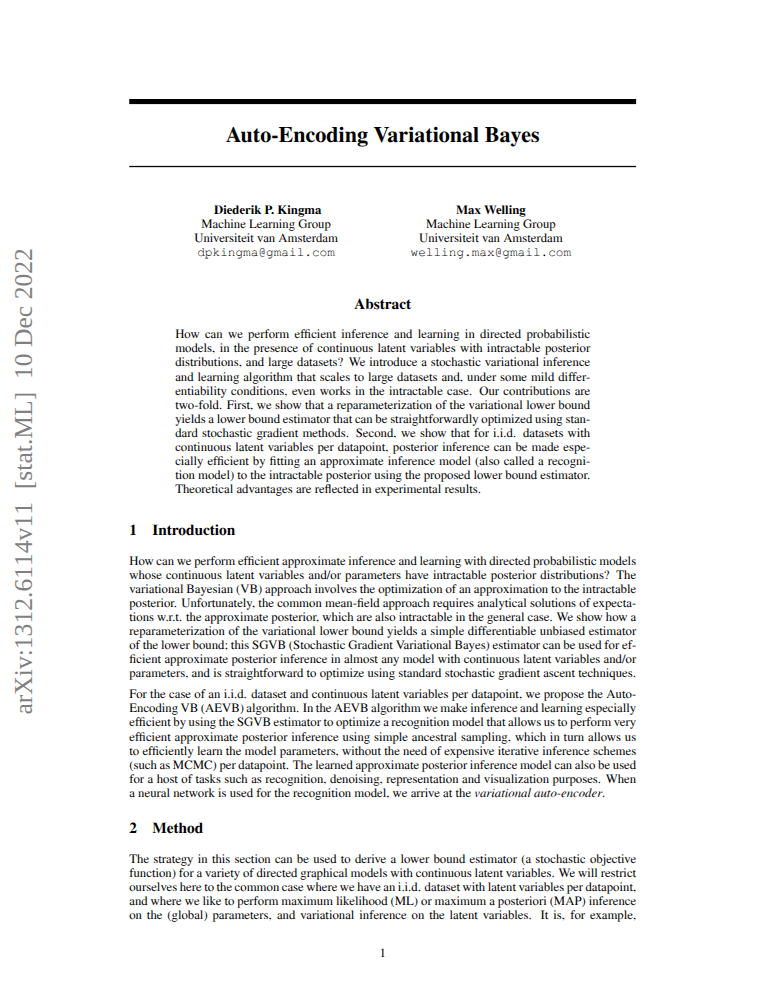
\includegraphics[height=0.9\textheight]{docs/slides/img/Screenshot from 2026-05-12 21-16-28.png}
\end{frame}

\begin{frame}
    \frametitle{Historical context}
    \begin{itemize}
        \setlength{\itemsep}{2em}
        \item VAE \cite{kingma2013auto} Arxived on Fri, 20 Dec 2013
        \item Similar \cite{rezende2014stochastic} published 27 days later
        \item 55k vs 7k citations \pause
        \item Lesson 1: don't get scooped \pause
        \item 2013: Adam, ResNets, BatchNorm/LayerNorm, etc don't yet exist
        \item VAEs relative to 2010s DL research:
    \end{itemize}
\end{frame}

\begin{frame}[shrink=20]
    \frametitle{Historical context}
    \begin{center}
        \begin{tabular}{l c l r}
            \hline
            \textbf{Contribution} & \textbf{Year} & \textbf{Reference} & \textbf{\# Citations} \\
            \hline
            ``Xavier''/``Glorot'' initialisation & 2010 & \cite{glorot2010understanding} & 30k \\
            AlexNet & 2012 & \cite{krizhevsky2012imagenet} & 155k \\
            Dropout & 2012 & \cite{hinton2012improving} & 13k \\
            \hline
            \hline
            \textbf{VAE} & \textbf{2013} & \textbf{\cite{kingma2013auto}} & \textbf{55k} \\
            \hline
            \hline
            VGGNet & 2014 & \cite{simonyan2014very} & 161k \\
            Adam & 2014 & \cite{kingma2014adam} & 243k \\
            Neural attention & 2014 & \cite{bahdanau2014neural} & 43k \\
            GANs & 2014 & \cite{goodfellow2014generative} & 94k \\
            BatchNorm & 2015 & \cite{ioffe2015batch} & 68k \\
            ResNet & 2015 & \cite{he2016deep} & 318k \\
            ``Kaiming''/``He'' initialisation & 2015 & \cite{he2015delving} & 30k \\
            Diffusion & 2015 & \cite{sohl2015deep} & 12k \\
            LayerNorm & 2016 & \cite{ba2016layer} & 19k \\
            Transformers & 2017 & \cite{vaswani2017attention} & 245k \\
            BERT & 2018 & \cite{devlin2019bert} & 168k \\
            GPT-1 & 2018 & \cite{radford2018improving} & 19k \\
            GPT-2 & 2019 & \cite{radford2019language} & 25k \\
            \hline
        \end{tabular}
    \end{center}
\end{frame}

\begin{frame}[t]
    \frametitle{VAE problem setting}
    \begin{itemize}
        \setlength{\itemsep}{0.8em}
        \item Observe data $x = \{x_1, \dots, x_N\}$
        \item Assume $x \sim p(x \,|\, \theta^*)$
        \item[$\bigstar$] Learn $\theta = \text{argmax}_\theta\Bigl[ \log\Bigl( p(x \,|\, \theta) \Bigr) \Bigr]$
        \item[$\bigstar$] Sample $\{x_{N+1}, \dots, x_{N+M}\}\sim p(x \,|\, \theta)$
        \item Model:
        \begin{itemize}
            \vspace{0.8em}
            \setlength{\itemsep}{0.8em}
            \item $\{x_1, \dots, x_N\}$ IID
            \item Sample $z_n \sim p\bigl( z_n \,\vert\, \theta \bigr)$
            \item Sample $x_n \sim p\bigl( x_n \,\vert\, z_n, \theta \bigr)$
            \item Observe $x_n$ \textcolor{black!40}{($z_n$ hidden)}
        \end{itemize}
    \end{itemize}
\end{frame}

\begin{frame}[t]
    \frametitle{VAE objective}
    \begin{itemize}
        \setlength{\itemsep}{0.5em}
        \item \emph{How} to learn $\theta = \text{argmax}_\theta\Bigl[ \log\Bigl( p(x \,|\, \theta) \Bigr) \Bigr]$ ?
        \begin{align*}
            & \log\Bigl( p\bigl(x \,\vert\, \theta\bigr) \Bigr) \tag{Log likelihood} \\
            &= \sum_{n=1}^N \left[ \log\Bigl( p\bigl(x_n \,\vert\, \theta\bigr) \Bigr) \right] \tag{IID} \\
            &= \sum_{n=1}^N \left[ \log\left( \int dz_n \Bigl[ p\bigl(x_n, z_n \,\vert\, \theta\bigr) \Bigr] \right) \right] \tag{Marginalise $z_n$} \\
            &= \sum_{n=1}^N \left[ \log\left( \int dz_n \Bigl[ p\bigl( z_n \,\vert\, \theta \bigr)\;p\bigl( x_n \,\vert\, z_n, \theta \bigr) \Bigr] \right) \right] \tag{Product rule $x_n | z_n$} \\
            &= \sum_{n=1}^N \left[ \log\left( \mathbb{E}_{p( z_n \,\vert\, \theta )} \Bigl[ p\bigl( x_n \,\vert\, z_n, \theta \bigr) \Bigr] \right) \right] \tag{$\int p = \mathbb{E}$}
        \end{align*}
    \end{itemize}
\end{frame}

\begin{frame}[t]
    \frametitle{VAE objective}
    \begin{itemize}
        \setlength{\itemsep}{0.5em}
        \item \emph{How} to learn $\theta = \text{argmax}_\theta\Bigl[ \log\Bigl( p(x \,|\, \theta) \Bigr) \Bigr]$ ?
        \begin{align*}
            \log\Bigl( p\bigl(x \,\vert\, \theta\bigr) \Bigr) &= \sum_{n=1}^N \left[ \log\left( \mathbb{E}_{p( z_n \,\vert\, \theta )} \Bigl[ p\bigl( x_n \,\vert\, z_n, \theta \bigr) \Bigr] \right) \right] \tag{Previous slide}
        \end{align*}
        \item Could:
        \begin{itemize}
            \vspace{0.5em}
            \setlength{\itemsep}{0.5em}
            \item Fix $p( z_n \,\vert\, \theta ) = \mathcal{N}(z_n \,|\, 0, I)$ and $p\bigl( x_n \,\vert\, z_n, \theta \bigr) = \text{MLP}$
            \item MC with $z_n \sim p( z_n \,\vert\, \theta )$
        \end{itemize}
        \item But:
        \begin{itemize}
            \vspace{0.5em}
            \setlength{\itemsep}{0.5em}
            \item Not unbiased ($\mathbb{E}$ inside log)
            \item p(sampled $z_n$ reconstructs $x_n$) = tiny $\Rightarrow$ need many samples
        \end{itemize}
        \item Instead choose* some $q(z_n \vert x_n, \phi) \approx p(z_n \vert x_n, \theta)$, maximise \emph{ELBO}
    \end{itemize}
\end{frame}

\begin{frame}[t]
    \frametitle{ELBO derivation}
    \begin{itemize}
        \item Expand log likelihood for each datapoint:
        \begin{align*}
            & \log\Bigl(p(x_n \vert \theta)\Bigr) \tag{Log likelihood} \\
            &= \int dz_n \left[ q(z_n \vert x_n, \phi) \log\Bigl(p(x_n \vert \theta)\Bigr) \right] \tag{Marginalise $q$} \\
            &= \int dz_n \left[ q(z_n \vert x_n, \phi) \log\left( \frac{p(x_n, z_n \vert \theta)}{p(z_n \vert x_n, \theta)} \right) \right] \tag{Product rule $z_n \vert x_n$} \\
            &= \int dz_n \biggl[ q(z_n \vert x_n, \phi) \log\left( \frac{p(x_n, z_n \vert \theta)}{q(z_n \vert x_n, \phi)} \right) \\
            &\qquad\quad + q(z_n \vert x_n, \phi) \log\left( \frac{q(z_n \vert x_n, \phi)}{p(z_n \vert x_n, \theta)} \right) \biggr] \tag{$\times\frac{q}{q}$}
        \end{align*}
    \end{itemize}
\end{frame}

\begin{frame}[t]
    \frametitle{ELBO derivation}
    \begin{align*}
        &= \int dz_n \biggl[ q(z_n \vert x_n, \phi) \log\left( \frac{p(x_n, z_n \vert \theta)}{q(z_n \vert x_n, \phi)} \right) \\
        &\qquad\quad + q(z_n \vert x_n, \phi) \log\left( \frac{q(z_n \vert x_n, \phi)}{p(z_n \vert x_n, \theta)} \right) \biggr] \tag{From previous slide} \\
        &= \int dz_n \biggl[ q(z_n \vert x_n, \phi) \log\left( \frac{p(x_n, z_n \vert \theta)}{q(z_n \vert x_n, \phi)} \right) \biggr] \\
        &\qquad\quad + \text{KL}\Bigl[q(z_n \vert x_n, \phi) \Bigm\Vert p(z_n \vert x_n, \theta)\Bigr] \tag{KL definition} \\
        &\ge \int dz_n \biggl[ q(z_n \vert x_n, \phi) \log\left( \frac{p(x_n, z_n \vert \theta)}{q(z_n \vert x_n, \phi)} \right) \biggr] \tag{KL $\ge 0$, ELBO v1}
    \end{align*}
\end{frame}

\begin{frame}
    \frametitle{ELBO derivation}
    \begin{align*}
        &\ge \int dz_n \biggl[ q(z_n \vert x_n, \phi) \log\left( \frac{p(x_n, z_n \vert \theta)}{q(z_n \vert x_n, \phi)} \right) \biggr] \tag{From previous slide} \\
        &= \int dz_n \biggl[ q(z_n \vert x_n, \phi) \log\left( \frac{p(z_n \vert \theta)}{q(z_n \vert x_n, \phi)} \right) \\
        &\qquad\quad + q(z_n \vert x_n, \phi) \log \Bigl( p(x_n \vert z_n, \theta) \Bigr) \biggr] \tag{Product rule* $x_n\vert z_n$} \\
        &= -\text{KL}\Bigl[q(z_n \vert x_n, \phi) \Bigm\Vert p(z_n \vert \theta)\Bigr] \\
        &\qquad + \mathbb{E}_{z_n\sim q(z_n \vert x_n, \phi)}\left[ \log \Bigl(p(x_n \vert z_n, \theta)\Bigr) \right] \tag{KL and $\mathbb{E}$ definitions} \\
        &= \mathcal{L}(x_n, \theta, \phi) \tag{ELBO, VAE version}
    \end{align*}
    \begin{itemize}
        \item NB $\mathcal{L}$ shorthand for ``ELBO'', not ``loss'' (we will maximise $\mathcal{L}$)
    \end{itemize}
\end{frame}

\begin{frame}
    \frametitle{ELBO interpretation}
    \begin{align*}
        \underbrace{\mathcal{L}(x_n, \theta, \phi)}_\text{Objective function} &= \textcolor{blue}{\underbrace{-\text{KL}\Bigl[q(z_n \vert x_n, \phi) \Bigm\Vert p(z_n \vert \theta)\Bigr]}_{\text{Regularise $z_n$}}} \\
        &\qquad + \textcolor{OliveGreen}{\underbrace{\mathbb{E}_{z_n\sim q(z_n \vert x_n, \phi)}\left[ \log \Bigl(p(x_n \vert z_n, \theta)\Bigr) \right]}_{\text{Reconstruct $x_n$}}} \tag{ELBO} \\
        &\le \log\Bigl(p(x_n \vert \theta)\Bigr) \tag{Log likelihood}
    \end{align*}
    \begin{itemize}
        \item Regularise $\Rightarrow$ don't overfit latent for every $x_n$
        \item Reconstruct $\Rightarrow$ learn accurate generative model
        \item Together $\Rightarrow$ new samples $z_n\sim p(z_n|\theta)$ decode to realistic $x_n$
    \end{itemize}
\end{frame}

\begin{frame}
    \frametitle{VAE challenges}
    \$1mQs:
    \begin{enumerate}
        \setlength{\itemsep}{2em}
        \vspace{2em}
        \item How to define $q(z_n \vert x_n, \phi)$ ?
        \item How to estimate $\frac{\partial\mathcal{L}}{\partial(\theta,\phi)}$ using BP?
    \end{enumerate}
\end{frame}

\begin{frame}
    \frametitle{VAE challenges}
    \$1mQs:
    \begin{enumerate}
        \setlength{\itemsep}{2em}
        \vspace{2em}
        \item How to define $q(z_n \vert x_n, \phi)$ ?
        \item \textcolor{black!30}{How to estimate $\frac{\partial\mathcal{L}}{\partial(\theta,\phi)}$ using BP?}
    \end{enumerate}
\end{frame}

\begin{frame}[t]
    \frametitle{Latent posterior}
    \begin{itemize}
        \setlength{\itemsep}{1em}
        \item How to choose $q(z_n \vert x_n, \phi)$ ?
        \item \emph{Could} learn some $q(z_n \vert x_n, \phi)$ separately for every $x_n$
        \begin{itemize}
            \setlength{\itemsep}{1em}
            \vspace{1em}
            \item $N$ large $\Rightarrow$ learn with batches
            \item Store all $q(z_n \vert x_n, \phi)$ in memory? $\Rightarrow$ Memory $O(N)$ \Sadey
            \item Learn $q(z_n \vert x_n, \phi)$ from scratch every iteration? Hard+wasteful \Sadey
        \end{itemize}
    \end{itemize}
\end{frame}

\begin{frame}[t]
    \frametitle{Latent posterior}
    \begin{itemize}
        \setlength{\itemsep}{1em}
        \item How to choose $q(z_n \vert x_n, \phi)$ ?
        \item \sout{\emph{Could} learn some $q(z_n \vert x_n, \phi)$ separately for every $x_n$}
        \item ``Amortised inference'' \Smiley
        \item EG:
        \begin{align*}
            (\mu, \sigma) &= \text{MLP}(x_n, \phi) \tag{MLP forward pass} \\
            q(z_n \,\vert\, x_n, \phi) &= \mathcal{N}\Bigl( z_n \Bigm\vert \mu, \text{diag}(\sigma)^2 \Bigr) \tag{Latent posterior}
        \end{align*}
        \item Cost ``amortised'' into $\phi$
        \item Learn good $\phi\;\Rightarrow$ have $q(z_n \vert x_n, \phi)$ for \emph{all} $x_n$ from MLP
        \item Assumptions: smooth $x_n \rightarrow p(z_n | x_n,\theta)$, MLPs generalise smoothly
    \end{itemize}
\end{frame}

\begin{frame}
    \frametitle{Recognition and generative models}
    \begin{itemize}
        \setlength{\itemsep}{0.5em}
        \item Recall ELBO:
        \begin{align*}
            \mathcal{L}(x_n, \theta, \phi) &= \textcolor{blue}{{-\text{KL}\Bigl[q(z_n \vert x_n, \phi) \Bigm\Vert p(z_n \vert \theta)\Bigr]}} \\
            &\qquad + \textcolor{OliveGreen}{\mathbb{E}_{z_n\sim q(z_n \vert x_n, \phi)}\left[ \log \Bigl(p(x_n \vert z_n, \theta)\Bigr) \right]} \tag{ELBO}
        \end{align*}
        \item 3 distributions: $p(z_n \vert \theta)$, $q(z_n \vert x_n, \phi)$, $p(x_n \vert z_n, \theta)$
        \item VAE:
        \begin{itemize}
            \setlength{\itemsep}{0.5em}
            \vspace{0.5em}
            \item $p(z_n \vert \theta)$ fixed, EG $\mathcal{N}(z_n | 0, I)$
            \item $q(z_n \vert x_n, \phi) =$ ``Encoder''/``Recognition'' model
            \item $p(x_n \vert z_n, \theta) =$ ``Decoder''/``Generative'' model
            \item Encoder, decoder = neural networks
        \end{itemize}
        \item NB recognition/generative terminology $\sim$ 18yo \cite{hinton1995wake}
    \end{itemize}
\end{frame}

\begin{frame}
    \frametitle{VAE challenges}
    \$1mQs:
    \begin{enumerate}
        \setlength{\itemsep}{2em}
        \vspace{2em}
        \item \sout{How to define $q(z_n \vert x_n, \phi)$ ?}
        \item How to estimate $\frac{\partial\mathcal{L}}{\partial(\theta,\phi)}$ using BP?
        \begin{enumerate}
            \setlength{\itemsep}{2em}
            \vspace{2em}
            \item KL term
            \item Reconstruction term
        \end{enumerate}
    \end{enumerate}
\end{frame}

\begin{frame}[t]
    \frametitle{Differentiating KL}
    \begin{itemize}
        \item Want to differentiate \textcolor{blue}{KL} term WRT $\phi$:
        \begin{align*}
            \mathcal{L}(x_n, \theta, \phi) &= -\textcolor{blue}{\text{KL}\Bigl[q(z_n \vert x_n, \phi) \Bigm\Vert p(z_n \vert \theta)\Bigr]} \\
            &\qquad + \mathbb{E}_{z_n\sim q(z_n \vert x_n, \phi)}\left[ \log \Bigl(p(x_n \vert z_n, \theta)\Bigr) \right] \tag{ELBO}
        \end{align*}
        \item Define encoder as diagonal Gaussian:
        \begin{align*}
            (\mu, \sigma) &= \text{MLP}_\text{enc}(x_n, \phi) \tag{Encoder forward} \\
            q(z_n \,\vert\, x_n, \phi) &= \mathcal{N}\Bigl( z_n \Bigm\vert \mu, \text{diag}(\sigma)^2 \Bigr) \tag{Encoder distribution}
        \end{align*}
        \item Assume:
        \begin{align*}
            p(z_n\vert\theta) = \mathcal{N}(z_n\vert 0, I) \tag{Prior distribution}
        \end{align*}
    \end{itemize}
\end{frame}

\begin{frame}[t]
    \frametitle{Differentiating KL}
    \begin{itemize}
        \item Want to differentiate \textcolor{blue}{KL} term WRT $\phi$:
        \begin{align*}
            \mathcal{L}(x_n, \theta, \phi) &= -\textcolor{blue}{\text{KL}\Bigl[q(z_n \vert x_n, \phi) \Bigm\Vert p(z_n \vert \theta)\Bigr]} \\
            &\qquad + \mathbb{E}_{z_n\sim q(z_n \vert x_n, \phi)}\left[ \log \Bigl(p(x_n \vert z_n, \theta)\Bigr) \right] \tag{ELBO}
        \end{align*}
        \hrule
        \begin{align*}
            q(z_n \,\vert\, x_n, \phi) &= \mathcal{N}\Bigl( z_n \Bigm\vert \mu, \text{diag}(\sigma)^2 \Bigr) \tag{Encoder distribution} \\
            p(z_n\vert\theta) &= \mathcal{N}(z_n\vert 0, I) \tag{Prior distribution} \\
        \end{align*}
        \begin{align*}
            \Rightarrow\quad &\textcolor{blue}{\text{KL}\Bigl[q(z_n \vert x_n, \phi) \Bigm\Vert p(z_n \vert \theta)\Bigr]} \\
            &= \mathbb{E}_{z_n\sim q(z_n \vert x_n, \phi)}\underbrace{\left[ \log \left(\frac{\mathcal{N}\Bigl( z_n \Bigm\vert \mu, \text{diag}(\sigma)^2 \Bigr)}{\mathcal{N}(z_n\vert 0, I)}\right) \right]}_\text{Quadratic in $z_n$} \\
        \end{align*}
    \end{itemize}
\end{frame}

\begin{frame}[t]
    \frametitle{Differentiating KL}
    \begin{itemize}
        \item Want to differentiate \textcolor{blue}{KL} term WRT $\phi$:
        \begin{align*}
            \mathcal{L}(x_n, \theta, \phi) &= -\textcolor{blue}{\text{KL}\Bigl[q(z_n \vert x_n, \phi) \Bigm\Vert p(z_n \vert \theta)\Bigr]} \\
            &\qquad + \mathbb{E}_{z_n\sim q(z_n \vert x_n, \phi)}\left[ \log \Bigl(p(x_n \vert z_n, \theta)\Bigr) \right] \tag{ELBO}
        \end{align*}
        \hrule
        \begin{align*}
            q(z_n \,\vert\, x_n, \phi) &= \mathcal{N}\Bigl( z_n \Bigm\vert \mu, \text{diag}(\sigma)^2 \Bigr) \tag{Encoder distribution} \\
            p(z_n\vert\theta) &= \mathcal{N}(z_n\vert 0, I) \tag{Prior distribution} \\
        \end{align*}
        \begin{align*}
            \Rightarrow\quad &\textcolor{blue}{\text{KL}\Bigl[q(z_n \vert x_n, \phi) \Bigm\Vert p(z_n \vert \theta)\Bigr]} \\
            &= \textcolor{blue}{-\frac{1}{2}\sum_i \Bigl[ 1 + 2\log(\sigma_i) - \mu_j^2 - \sigma_j^2 \Bigr]} \tag{\textcolor{blue}{Closed-form KL \Smiley}}
        \end{align*}
    \end{itemize}
\end{frame}

\begin{frame}
    \frametitle{VAE challenges}
    \$1mQs:
    \begin{enumerate}
        \setlength{\itemsep}{2em}
        \vspace{2em}
        \item \sout{How to define $q(z_n \vert x_n, \phi)$ ?}
        \item How to estimate $\frac{\partial\mathcal{L}}{\partial(\theta,\phi)}$ using BP?
        \begin{enumerate}
            \setlength{\itemsep}{2em}
            \vspace{2em}
            \item \sout{KL term}
            \item Reconstruction term
        \end{enumerate}
    \end{enumerate}
\end{frame}

\begin{frame}[t]
    \frametitle{Score function estimator?}
    \begin{itemize}
        \item Want to differentiate \textcolor{OliveGreen}{reconstruction} term WRT $\phi$:
        \begin{align*}
            \mathcal{L}(x_n, \theta, \phi) &= -\text{KL}\Bigl[q(z_n \vert x_n, \phi) \Bigm\Vert p(z_n \vert \theta)\Bigr] \\
            &\qquad + \textcolor{OliveGreen}{\mathbb{E}_{z_n\sim q(z_n \vert x_n, \phi)}\left[ \log \Bigl(p(x_n \vert z_n, \theta)\Bigr) \right]} \tag{ELBO}
        \end{align*}
        \item \emph{Can} differentiate using SFE:
        \begin{align*}
            &\frac{\partial}{\partial \phi}\Biggl[\textcolor{OliveGreen}{\mathbb{E}_{z_n\sim q(z_n \vert x_n, \phi)}\biggl[ \log \Bigl(p(x_n \vert z_n, \theta)\Bigr) \biggr]}\Biggr] \\
            &= \frac{\partial}{\partial \phi}\Biggl[\int dz_n \biggl[ q(z_n \vert x_n, \phi) \log \Bigl(p(x_n \vert z_n, \theta)\Bigr) \biggr]\Biggr] \tag{$\mathbb{E}=\int q$} \\
            &= \int dz_n \Biggl[ \frac{\partial}{\partial \phi}\Bigl[q(z_n \vert x_n, \phi)\Bigr] \log \Bigl(p(x_n \vert z_n, \theta)\Bigr) \Biggr] \tag{Swap $\partial$ and $\int$}
        \end{align*}
    \end{itemize}
\end{frame}

\begin{frame}[t]
    \frametitle{Score function estimator?}
    \begin{align*}
        &= \int dz_n \Biggl[ \frac{\partial}{\partial \phi}\Bigl[q(z_n \vert x_n, \phi)\Bigr] \log \Bigl(p(x_n \vert z_n, \theta)\Bigr) \Biggr] \tag{From previous slide} \\
        &= \int dz_n \Biggl[ q(z_n \vert x_n, \phi) \frac{\frac{\partial}{\partial \phi}\Bigl[q(z_n \vert x_n, \phi)\Bigr]}{q(z_n \vert x_n, \phi)} \log \Bigl(p(x_n \vert z_n, \theta)\Bigr) \Biggr] \tag{$\times\frac{q}{q}$} \\
        &= \int dz_n \Biggl[ q(z_n \vert x_n, \phi) \frac{\partial}{\partial \phi}\biggl[\log \Bigl(q(z_n \vert x_n, \phi)\Bigr)\biggr] \log \Bigl(p(x_n \vert z_n, \theta)\Bigr) \Biggr] \tag{$\frac{\nabla[q]}{q}=\nabla\bigl[\log(q)\bigr]$} \\
        &= \mathbb{E}_{z_n\sim q(z_n \vert x_n, \phi)} \Biggl[ \frac{\partial}{\partial \phi}\biggl[\log \Bigl(q(z_n \vert x_n, \phi)\Bigr)\biggr] \log \Bigl(p(x_n \vert z_n, \theta)\Bigr) \Biggr] \tag{$\int q=\mathbb{E}$} \\
    \end{align*}
\end{frame}

\begin{frame}[t]
    \frametitle{Score function estimator?}
    \begin{align*}
        \Rightarrow\quad &\frac{\partial}{\partial \phi}\Biggl[\textcolor{OliveGreen}{\mathbb{E}_{z_n\sim q(z_n \vert x_n, \phi)}\biggl[ \log \Bigl(p(x_n \vert z_n, \theta)\Bigr) \biggr]}\Biggr] \\
        &= \mathbb{E}_{z_n\sim q(z_n \vert x_n, \phi)} \Biggl[ \frac{\partial}{\partial \phi}\biggl[\log \Bigl(q(z_n \vert x_n, \phi)\Bigr)\biggr] \log \Bigl(p(x_n \vert z_n, \theta)\Bigr) \Biggr] \tag{SFE} \label{eq:SFE}
    \end{align*}
    \begin{itemize}
        \setlength{\itemsep}{1em}
        \item \emph{Can} MC and evaluate (\ref{eq:SFE}) with BP
        \item \emph{But} (\ref{eq:SFE}) ``exhibits very high variance'' \cite{kingma2013auto}
        \begin{itemize}
            \vspace{1em}
            \item (Empirical comparison?)
        \end{itemize}
    \end{itemize}
\end{frame}

\begin{frame}[t]
    \frametitle{\sout{Score function estimator?} Reparameterisation trick!}
    \begin{itemize}
        \item Want to differentiate \textcolor{OliveGreen}{reconstruction} term WRT $\phi$:
        \begin{align*}
            \mathcal{L}(x_n, \theta, \phi) &= -\text{KL}\Bigl[q(z_n \vert x_n, \phi) \Bigm\Vert p(z_n \vert \theta)\Bigr] \\
            &\qquad + \textcolor{OliveGreen}{\mathbb{E}_{z_n\sim q(z_n \vert x_n, \phi)}\left[ \log \Bigl(p(x_n \vert z_n, \theta)\Bigr) \right]} \tag{ELBO}
        \end{align*}
        \item Recall encoder = diagonal Gaussian:
        \begin{align*}
            (\mu, \sigma) &= \text{MLP}_\text{enc}(x_n, \phi) \tag{Encoder forward} \\
            q(z_n \,\vert\, x_n, \phi) &= \mathcal{N}\Bigl( z_n \Bigm\vert \mu, \text{diag}(\sigma)^2 \Bigr) \tag{Encoder distribution}
        \end{align*}
        \item ``Reparameterise'' $z_n$ as transform of auxiliary noise variable $\varepsilon$:
        \begin{align*}
            \varepsilon &\sim \mathcal{N}(\varepsilon \vert 0, I) \tag{Auxiliary noise sample} \\
            z_n &= \mu + \varepsilon \odot \sigma \tag{Reparameterisation trick} \\
            \Rightarrow\quad z_n &\sim q(z_n \vert x_n, \phi) \tag{Desired latent sample}
        \end{align*}
    \end{itemize}
\end{frame}

\begin{frame}[t]
    \frametitle{\sout{Score function estimator?} Reparameterisation trick!}
    \begin{itemize}
        \item Want to differentiate \textcolor{OliveGreen}{reconstruction} term WRT $\phi$:
        \begin{align*}
            \mathcal{L}(x_n, \theta, \phi) &= -\text{KL}\Bigl[q(z_n \vert x_n, \phi) \Bigm\Vert p(z_n \vert \theta)\Bigr] \\
            &\qquad + \textcolor{OliveGreen}{\mathbb{E}_{z_n\sim q(z_n \vert x_n, \phi)}\left[ \log \Bigl(p(x_n \vert z_n, \theta)\Bigr) \right]} \tag{ELBO}
        \end{align*}
    \end{itemize}
    \hrule
    \begin{align*}
        \Rightarrow\quad & \frac{\partial}{\partial\phi}\biggl[\textcolor{OliveGreen}{\mathbb{E}_{z_n\sim q(z_n \vert x_n, \phi)}\left[ \log \Bigl(p(x_n \vert z_n, \theta)\Bigr) \right]}\biggr] \\
        &= \frac{\partial}{\partial\phi}\Biggl[\mathbb{E}_{\varepsilon \sim \mathcal{N}(\varepsilon \vert 0, I)}\left[ \log \biggl(p\Bigl(x_n \Bigm\vert \mu + \varepsilon \odot \sigma, \theta\Bigr)\biggr) \right]\Biggr] \tag{Reparameterise} \\
        &= \mathbb{E}_{\varepsilon \sim \mathcal{N}(\varepsilon \vert 0, I)}\Biggl[\frac{\partial}{\partial\phi}\left[ \log \biggl(p\Bigl(x_n \Bigm\vert \mu + \varepsilon \odot \sigma, \theta\Bigr)\biggr) \right]\Biggr] \tag{Swap $\partial$ and $\mathbb{E}$} \\
        &\approx \frac{1}{L}\sum_{l=1}^L\Biggl[\frac{\partial}{\partial\phi}\left[ \log \biggl(p\Bigl(x_n \Bigm\vert \mu + \varepsilon^{(l)} \odot \sigma, \theta\Bigr)\biggr) \right]\Biggr] \tag{MC}
    \end{align*}
\end{frame}

\begin{frame}
    \frametitle{Evaluating reconstruction term}
    \begin{align*}
        & \textcolor{OliveGreen}{\mathbb{E}_{z_n\sim q(z_n \vert x_n, \phi)}\left[ \log \Bigl(p(x_n \vert z_n, \theta)\Bigr) \right]} \\
        &\approx \frac{1}{L}\sum_{l=1}^L\left[ \log \biggl(p\Bigl(x_n \Bigm\vert \mu + \varepsilon^{(l)} \odot \sigma, \theta\Bigr)\biggr) \right] \tag{Reconstruction term}
    \end{align*}
    \begin{itemize}
        \setlength{\itemsep}{0.5em}
        \item Large batch size $\Rightarrow$ can set $L=1$ \cite{kingma2013auto}
        \item Freedom to choose $p(x_n\vert z_n,\theta)$
        \item EG $x_n$ is continuous $\Rightarrow$ diagonal Gaussian:
    \end{itemize}
    \begin{align*}
        \left(\mu^{(x)}, \sigma^{(x)}\right) &= \text{MLP}_\text{dec}(z_n, \theta) \tag{Decoder forward} \\
        p(x_n \,\vert\, z_n, \theta) &= \mathcal{N}\left( x_n \;\middle\vert\; \mu^{(x)}, \text{diag}\left(\sigma^{(x)}\right)^2 \right) \tag{Decoder distribution}
    \end{align*}
\end{frame}

\begin{frame}
    \frametitle{Evaluating reconstruction term}
    \begin{align*}
        &\log\Bigl( p(x_n \,\vert\, z_n, \theta) \Bigr) \\
        &= \log\Biggl(\mathcal{N}\left( x_n \;\middle\vert\; \mu^{(x)}, \text{diag}\left(\sigma^{(x)}\right)^2 \right) \tag{Decoder log likelihood}\Biggr) \\
        &= \log\left( \prod_i\left[ \frac{1}{\sqrt{2\pi}\sigma^{(x)}_i} \exp\left(-\frac{1}{2}\left(\frac{x_{ni}-\mu^{(x)}_i}{\sigma^{(x)}_i}\right)^2\right) \right] \right) \tag{$\mathcal{N}$ definition} \\
        &= \frac{1}{2}\sum_i\left[ -\log(2\pi) - 2\log\left( \sigma^{(x)}_i \right) - \left(\frac{x_{ni}-\mu^{(x)}_i}{\sigma^{(x)}_i}\right)^2 \right] \tag{Expand logs}
    \end{align*}
\end{frame}

\begin{frame}
    \frametitle{Evaluating reconstruction term}
    \begin{align*}
        \Rightarrow\quad & \textcolor{OliveGreen}{\mathbb{E}_{z_n\sim q(z_n \vert x_n, \phi)}\left[ \log \Bigl(p(x_n \vert z_n, \theta)\Bigr) \right]} \\
        &\approx \frac{1}{2}\sum_i\left[ -\log(2\pi) - 2\log\left( \sigma^{(x)}_i \right) - \left(\frac{x_{ni}-\mu^{(x)}_i}{\sigma^{(x)}_i}\right)^2 \right] \tag{$\mathcal{N},L=1$}
    \end{align*}
    \begin{itemize}
        \item Putting this together\dots
    \end{itemize}
\end{frame}

\begin{frame}
    \frametitle{ELBO estimator}
    \begin{itemize}
        \item Now we have a differentiable + unbiased ELBO estimator \Smiley
    \end{itemize}
    \begin{align*}
        \mathcal{L}(x_n, \theta, \phi) &= \textcolor{blue}{{-\text{KL}\Bigl[q(z_n \vert x_n, \phi) \Bigm\Vert p(z_n \vert \theta)\Bigr]}} \\
        &\qquad + \textcolor{OliveGreen}{\mathbb{E}_{z_n\sim q(z_n \vert x_n, \phi)}\left[ \log \Bigl(p(x_n \vert z_n, \theta)\Bigr) \right]} \tag{ELBO} \\
        \\
        \widehat{\mathcal{L}}(x_n, \theta, \phi) &= \textcolor{blue}{\frac{1}{2}\sum_i \Bigl[ 1 + 2\log(\sigma_i) - \mu_j^2 - \sigma_j^2 \Bigr]} \\
        &\qquad + \textcolor{OliveGreen}{\frac{1}{2}\sum_i\left[ -\log(2\pi) - 2\log\left( \sigma^{(x)}_i \right) - \left(\frac{x_{ni}-\mu^{(x)}_i}{\sigma^{(x)}_i}\right)^2 \right]} \tag{Estimator}
    \end{align*}
\end{frame}

\begin{frame}
    \frametitle{VAE training algorithm}
    \begin{itemize}
        \item For each batch of data $\{x_1,x_2,\dots\}$:
        \begin{itemize}
            \item For each element $x_n$ in the batch:
        \end{itemize}
    \end{itemize}
    \begin{align*}
        (\mu, \sigma) &= \text{MLP}_\text{enc}(x_n, \phi) \tag{Encoder forward} \\
        \varepsilon &\sim \mathcal{N}(\varepsilon \vert 0, I) \tag{Auxiliary noise sample} \\
        z_n &= \mu + \varepsilon \odot \sigma \tag{Reparameterise} \\
        \left(\mu^{(x)}, \sigma^{(x)}\right) &= \text{MLP}_\text{dec}(z_n, \theta) \tag{Decoder forward} \\
        \widehat{\mathcal{L}}(x_n, \theta, \phi) &= \textcolor{blue}{\frac{1}{2}\sum_i \Bigl[ 1 + 2\log(\sigma_i) - \mu_j^2 - \sigma_j^2 \Bigr]} \\
        &\qquad + \textcolor{OliveGreen}{\frac{1}{2}\sum_i\left[ -\log(2\pi) - 2\log\left( \sigma^{(x)}_i \right) - \left(\frac{x_{ni}-\mu^{(x)}_i}{\sigma^{(x)}_i}\right)^2 \right]} \tag{$\widehat{\text{ELBO}}$}
    \end{align*}
\end{frame}

\begin{frame}
    \frametitle{VAE training algorithm}
    \begin{itemize}
        \item For each batch of data $\{x_1,x_2,\dots\}$:
        \begin{itemize}
            \item For each element $x_n$ in the batch:
        \end{itemize}
    \end{itemize}
    \begin{align*}
        \widehat{\mathcal{L}}(x_n, \theta, \phi) &= \textcolor{blue}{\frac{1}{2}\sum_i \Bigl[ 1 + 2\log(\sigma_i) - \mu_j^2 - \sigma_j^2 \Bigr]} \\
        &\qquad + \textcolor{OliveGreen}{\frac{1}{2}\sum_i\left[ -\log(2\pi) - 2\log\left( \sigma^{(x)}_i \right) - \left(\frac{x_{ni}-\mu^{(x)}_i}{\sigma^{(x)}_i}\right)^2 \right]} \tag{$\widehat{\text{ELBO}}$} \\
        (\theta, \phi) &\leftarrow (\theta, \phi) - \frac{\partial}{\partial (\theta, \phi)} \left[\sum_n \Bigl[ -\widehat{\mathcal{L}}(x_n, \theta, \phi) \Bigr]\right] \tag{SGD}
    \end{align*}
\end{frame}

\begin{frame}
    \frametitle{VAE sampling algorithm}
    \begin{align*}
        z&\sim \mathcal{N}(z\vert 0, I) \tag{Sample latent from prior} \\
        \left(\mu^{(x)}, \sigma^{(x)}\right) &= \text{MLP}_\text{dec}(z, \theta) \tag{Decoder forward} \\
        \varepsilon &\sim \mathcal{N}(\varepsilon \vert 0, I) \tag{Auxiliary noise samples} \\
        x &= \mu^{(x)} + \varepsilon \odot \sigma^{(x)} \tag{Reparameterise} \\
    \end{align*}
    \vfill
    \begin{itemize}
        \setlength{\itemsep}{1em}
        \item NB don't use $q$ or $\phi$ during sampling
        \item Simple, non-iterative, no extra HPs
    \end{itemize}
\end{frame}

\begin{frame}
    \frametitle{VAE summary}
    \begin{itemize}
        \setlength{\itemsep}{1em}
        \item 3 tricks (2 established, 1 innovation*):
        \begin{itemize}
            \setlength{\itemsep}{0.5em}
            \vspace{0.5em}
            \item $\text{argmax}_\theta\Bigl[p(x|\theta)\Bigr] \rightarrow \text{argmax}_\theta\bigl[\text{ELBO}\bigr]$
            \item Amortised inference $q(z_n | x_n, \theta)$
            \item Reparameterisation trick* $z_n = \mu + \varepsilon \odot \sigma$
        \end{itemize}
        \item Fits into \emph{now-standard} (then-visionary) DL framework:
        \begin{itemize}
            \setlength{\itemsep}{0.5em}
            \vspace{0.5em}
            \item Define model(s) + $\mathcal{L}$
            \item $\partial/\partial x$ (BP)
            \item SGD
        \end{itemize}
    \end{itemize}
\end{frame}

\begin{frame}
    \frametitle{Results \cite{kingma2013auto}}
    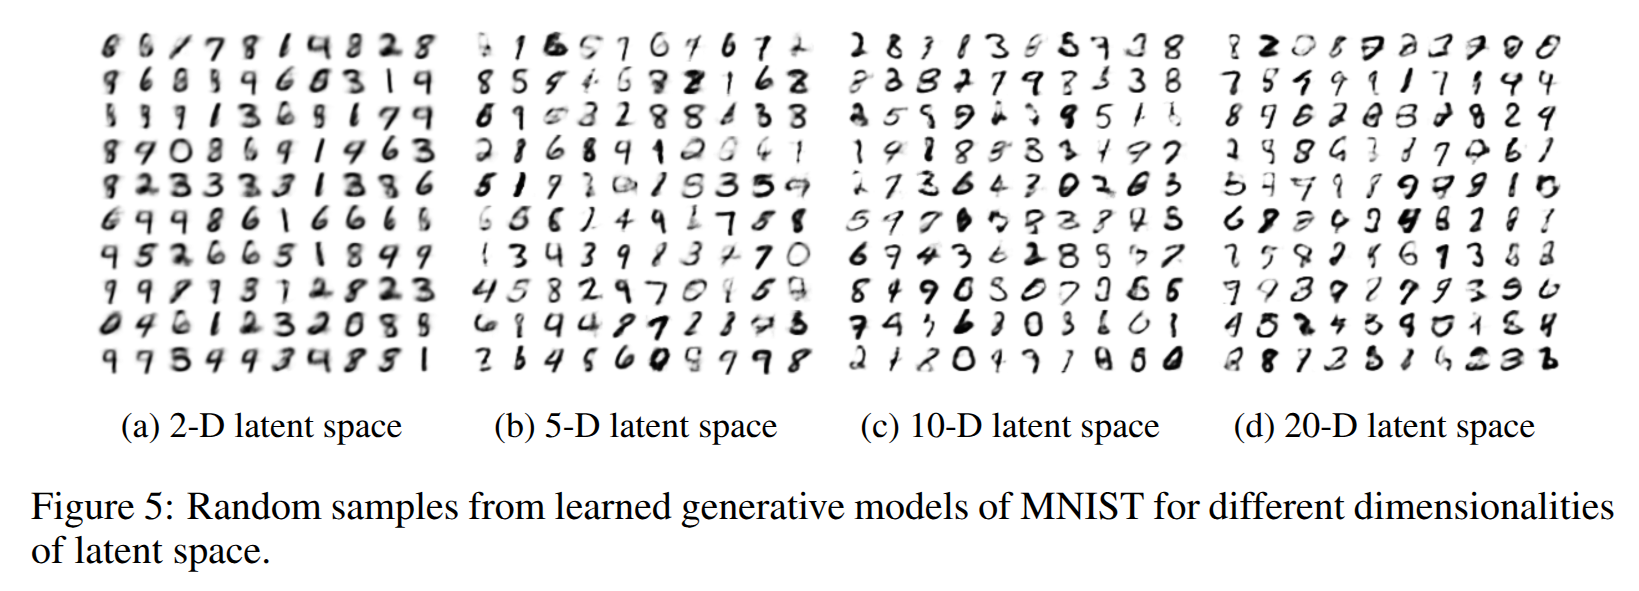
\includegraphics[width=\textwidth]{docs/slides/img/Screenshot from 2026-05-09 11-24-04.png}
\end{frame}

\begin{frame}
    \frametitle{Results \cite{kingma2013auto}}
    \centering
    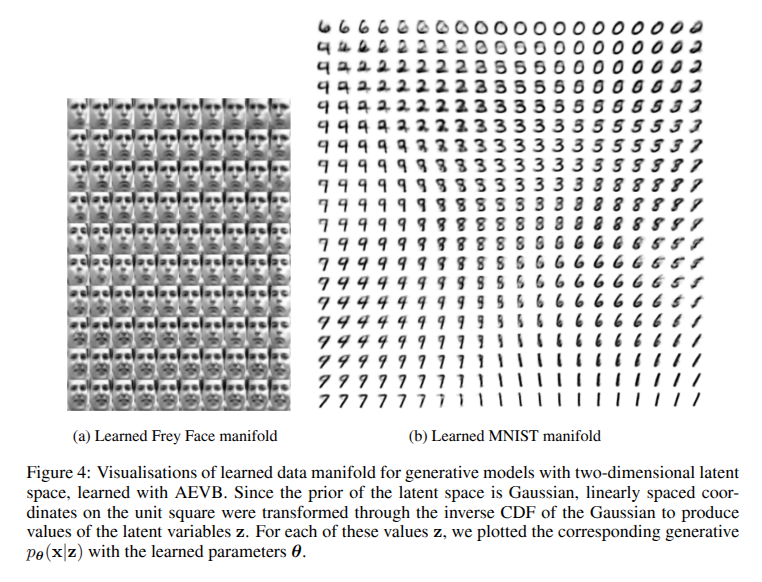
\includegraphics[height=0.8\textheight]{docs/slides/img/Screenshot from 2026-05-09 11-24-54.png}
\end{frame}

\begin{frame}
    \frametitle{VAE demo}
    \begin{itemize}
        \item VAE implementation: \url{https://github.com/jakelevi1996/vae/blob/main/src/vae/models/vae.py}
    \end{itemize}
\end{frame}

\begin{frame}
    \frametitle{VAE demo 2D dataset results}
    \begin{figure}
        \hfill
        \begin{subfigure}{0.3\textwidth}
            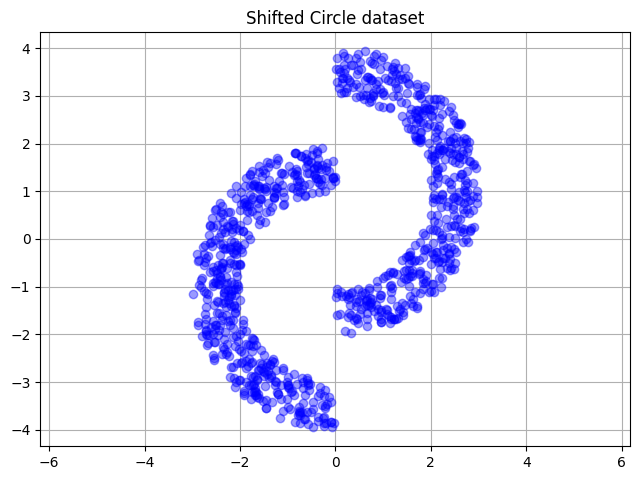
\includegraphics[width=\textwidth]{results/Shifted_Circle_dataset.png}
            \caption{Dataset}
        \end{subfigure}
        \hfill
        \begin{subfigure}{0.45\textwidth}
            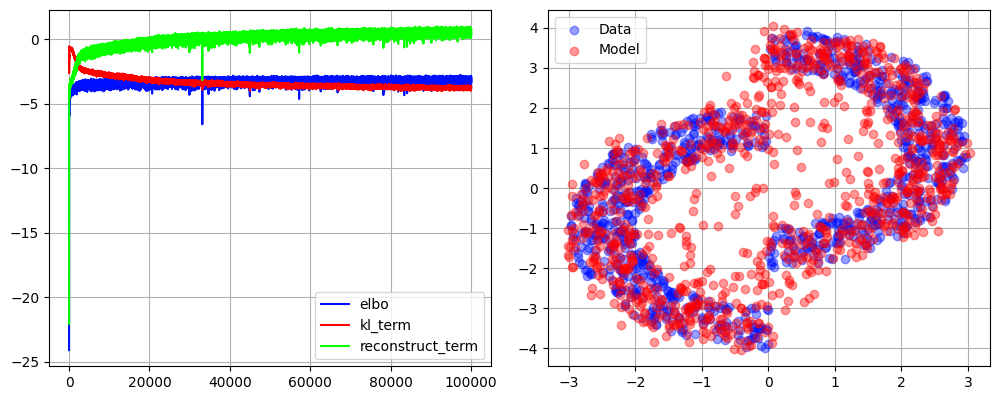
\includegraphics[width=\textwidth]{results/train_vae_circle/output.png}
            \caption{Seed = 0}
        \end{subfigure}
        \hfill
        \newline
        \vfill
        \begin{subfigure}{0.45\textwidth}
            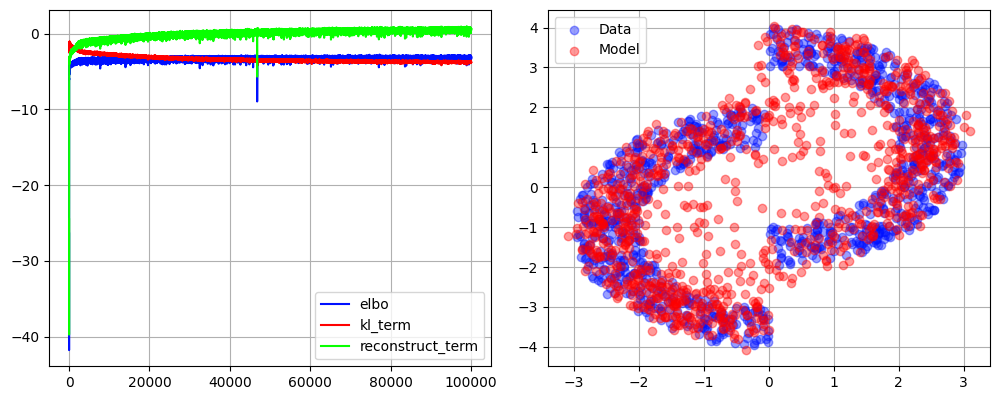
\includegraphics[width=\textwidth]{results/train_vae_circle/s1/output.png}
            \caption{Seed = 1}
        \end{subfigure}
        \hfill
        \begin{subfigure}{0.45\textwidth}
            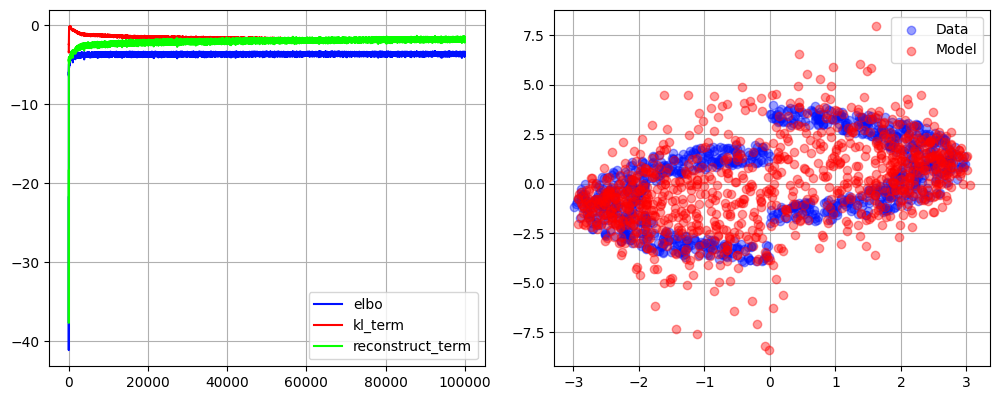
\includegraphics[width=\textwidth]{results/train_vae_circle/s2/output.png}
            \caption{Seed = 2}
        \end{subfigure}
    \end{figure}
\end{frame}

\begin{frame}
    \frametitle{VAE demo 2D dataset results}
    \begin{itemize}
        \item Example with learned shared $\sigma$ (not from MLP):
    \end{itemize}
    \vfill
    \centering
    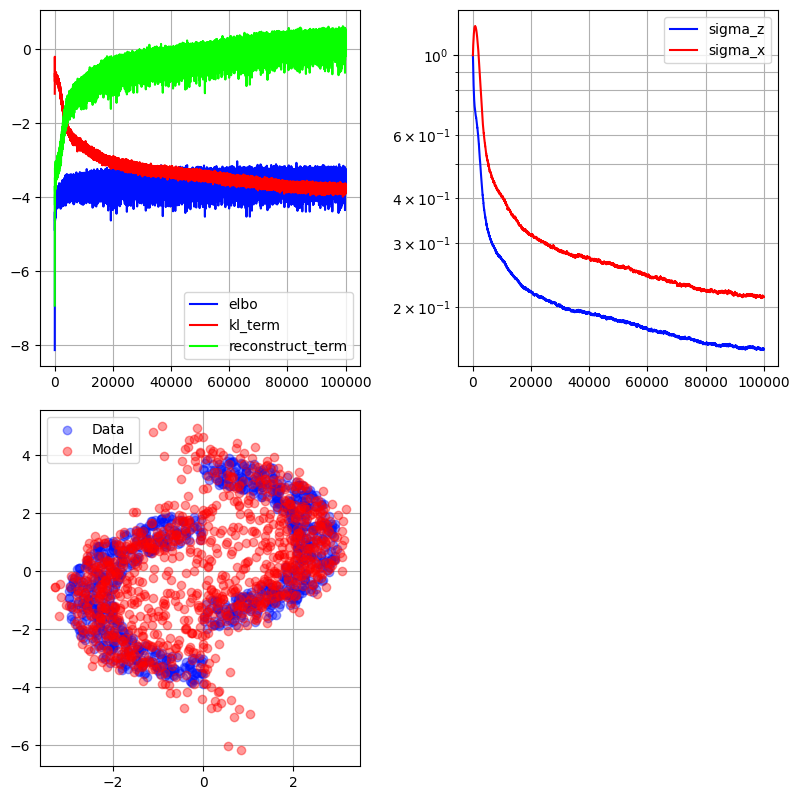
\includegraphics[height=0.6\textheight]{results/train_vae_circle_shared_sigma/s0/output_copy.png}
\end{frame}

\begin{frame}
    \frametitle{VAE MNIST demo}
    \centering
    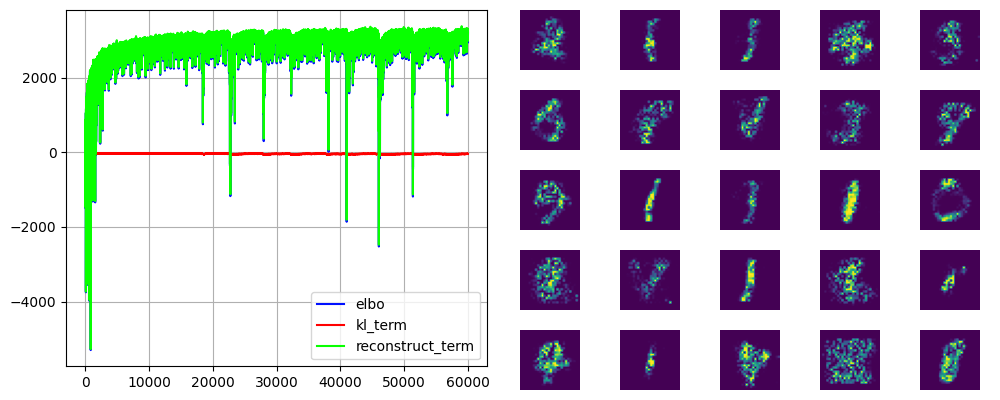
\includegraphics[width=\textwidth]{results/train_vae_mnist/e100s0/output.png}
\end{frame}

\begin{frame}
    \frametitle{VAE MNIST demo}
    \begin{itemize}
        \setlength{\itemsep}{1.8em}
        \item NB for MNIST:
        \begin{itemize}
            \vspace{0.5em}
            \setlength{\itemsep}{1em}
            \item Above demo = 100 epochs $\approx$ 30 minutes \pause
            \item \cite{kingma2013auto} train for $>$1000 epochs/33 hours !!!
            \item Classification: 5 epochs $\Rightarrow$ $<$30 seconds $\Rightarrow$ $>$98\% test acc
            \item Discriminative VS generative?
        \end{itemize}
    \end{itemize}
\end{frame}

\begin{frame}
    \frametitle{What's next?}
    \begin{enumerate}
        \setlength{\itemsep}{1.5em}
        \item Conditional generation \cite{kingma2014semi, sohn2015learning, yan2016attribute2image}
        \item Molecule generation \cite{gomez2018automatic, jin2018junction, griffiths2020constrained, grosnit2021high, maus2022local, sevgen2025prot}
        \item Object-centric learning \cite{watters2019spatial, burgess2019monet, locatello2020object}
        \item Discrete latent variables \cite{jang2016categorical, maddison2016concrete, van2017neural}
        \item \dots
    \end{enumerate}
\end{frame}

\begin{frame}
    \frametitle{M2}
    \centering
    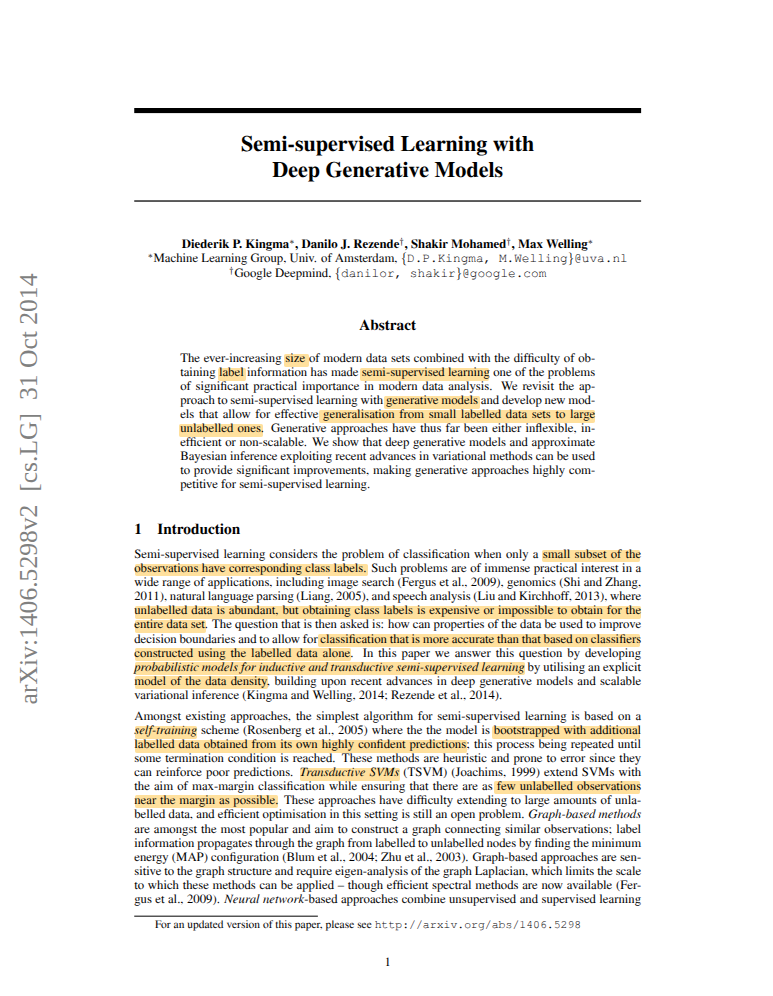
\includegraphics[height=0.9\textheight]{docs/slides/img/Screenshot from 2026-05-09 22-22-49.png}
\end{frame}

\begin{frame}
    \frametitle{M2}
    \begin{itemize}
        \setlength{\itemsep}{1em}
        \item \cite{kingma2014semi}
        \item Semi-supervised learning:
        \begin{itemize}
            \item LARGE unlabelled dataset $\{x_i, \dots\}\sim\tilde{p}_u$
            \item small labelled dataset $\{(x_j, y_j), \dots\}\sim\tilde{p}_l$
            \item Train classifier
            \item Outperform ignoring $\{x_i, \dots\}$
        \end{itemize}
        \item 3 models proposed:
        \begin{itemize}
            \item M1 = train VAE on $x$, train classifier on $y$ from $z$
            \item M2 (next slide)
            \item M1+M2 = use $z$ from M1 as $x$ for M2
        \end{itemize}
    \end{itemize}
\end{frame}

\begin{frame}
    \frametitle{M2}
    \begin{itemize}
        \item Model:
        \begin{align*}
            p_\theta(x, y, z) &= p_\theta(x\vert y, z)\;p(y)\;p(z) \tag{Generative model} \\
            q_\phi (z, y\vert x) &= q_\phi (z\vert x) \; q_\phi (y\vert x) \tag{Factorised posterior}
        \end{align*}
        \item Different loss functions for with/without labels:
        \item With labels:
        \begin{align*}
            \log\Bigl( p(x, y) \Bigr) &\ge \mathbb{E}_{q_\phi(z\vert x)}\left[ \log\left(\frac{p(x, y, z)}{q_\phi(z\vert x)}\right) \right] \\
            &= \mathbb{E}_{q_\phi(z\vert x)}\biggl[ \log\Bigl( p_\theta(x \vert y, z) \Bigr) + \log\Bigl( p(y) \Bigr) \\
            &\qquad\qquad + \log\Bigl( p(z) \Bigr) - \log\Bigl( q_\phi(z\vert x) \Bigr) \biggr] \\
            &= -\mathcal{L}(x, y)
        \end{align*}
    \end{itemize}
\end{frame}

\begin{frame}
    \frametitle{M2}
    \begin{itemize}
        \item With label:
        \begin{align*}
            -\mathcal{L}(x, y) &= \mathbb{E}_{q_\phi(z\vert x)}\biggl[ \log\Bigl( p_\theta(x \vert y, z) \Bigr) + \log\Bigl( p(y) \Bigr) \\
            &\qquad\qquad + \log\Bigl( p(z) \Bigr) - \log\Bigl( q_\phi(z\vert x) \Bigr) \biggr]
        \end{align*}
        \item Without label:
        \begin{align*}
            \log\Bigl( p(x) \Bigr) &\ge \mathbb{E}_{q_\phi(y, z\vert x)}\left[ \log\left(\frac{p(x, y, z)}{q_\phi(y, z\vert x)}\right) \right] \\
            &= \mathbb{E}_{q_\phi(y\vert x)}\biggl[ \mathbb{E}_{q_\phi(z\vert x)}\biggl[ \log\Bigl( p_\theta(x \vert y, z) \Bigr) + \log\Bigl( p(y) \Bigr) \\
            &\qquad\qquad + \log\Bigl( p(z) \Bigr) - \log\Bigl( q_\phi(z\vert x) \Bigr) - \log\Bigl( q_\phi(y\vert x) \Bigr) \biggr] \biggr] \\
            &= \mathbb{E}_{q_\phi(y\vert x)} \Bigl[-\mathcal{L}(x, y)\Bigr] + \mathcal{H}\Bigl[ q_\phi(y\vert x) \Bigr]
        \end{align*}
    \end{itemize}
\end{frame}

\begin{frame}
    \frametitle{M2}
    \begin{itemize}
        \item With label:
        \begin{align*}
            -\mathcal{L}(x, y) &= \mathbb{E}_{q_\phi(z\vert x)}\biggl[ \log\Bigl( p_\theta(x \vert y, z) \Bigr) + \log\Bigl( p(y) \Bigr) \\
            &\qquad\qquad + \log\Bigl( p(z) \Bigr) - \log\Bigl( q_\phi(z\vert x) \Bigr) \biggr]
        \end{align*}
        \item Without label:
        \begin{align*}
            -\mathcal{U}(x) &= \mathbb{E}_{q_\phi(y\vert x)} \Bigl[-\mathcal{L}(x, y)\Bigr] + \mathcal{H}\Bigl[ q_\phi(y\vert x) \Bigr]
        \end{align*}
        \item Bound on ML for full dataset:
        \begin{align*}
            \mathcal{J} &= \sum_{(x, y)\sim\tilde{p}_l} \Bigl[ \mathcal{L}(x, y) \Bigr] + \sum_{x\sim\tilde{p}_u} \Bigl[ \mathcal{U}(x) \Bigr]
        \end{align*}
        \item Total loss: + term to train classifier $q_\phi(y\vert x)$ on $(x, y)\sim\tilde{p}_l$
    \end{itemize}
\end{frame}

\begin{frame}
    \frametitle{M2}
    \begin{itemize}
        \item Semi-supervised classification results:
    \end{itemize}
    \vfill
    \centering
    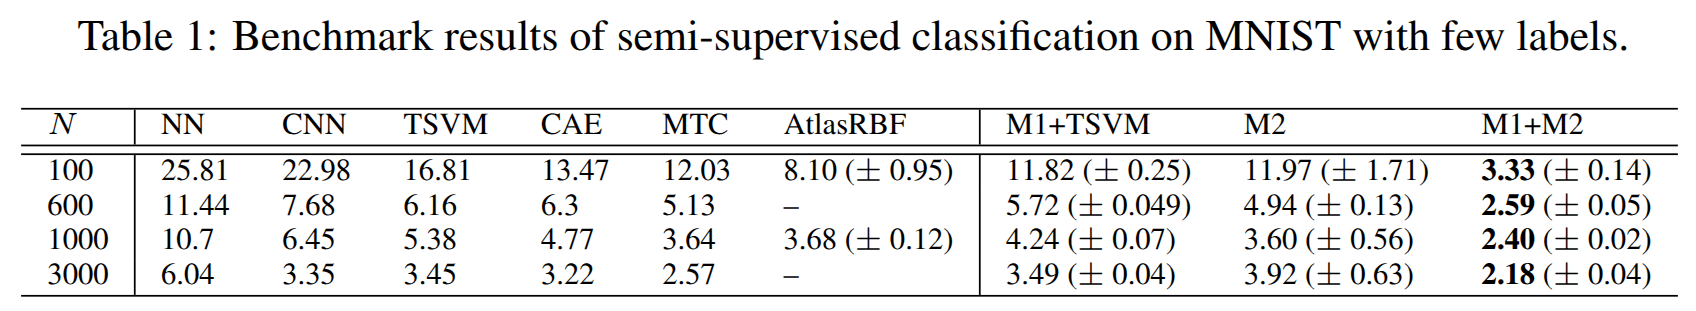
\includegraphics[width=\textwidth]{docs/slides/img/Screenshot from 2026-05-09 23-10-35.png}
\end{frame}

\begin{frame}
    \frametitle{M2}
    \frametitle{M2}
    \begin{itemize}
        \item Using $p_\theta(x \vert y, z)$, fixing $y/z$ respectively:
    \end{itemize}
    \vfill
    \centering
    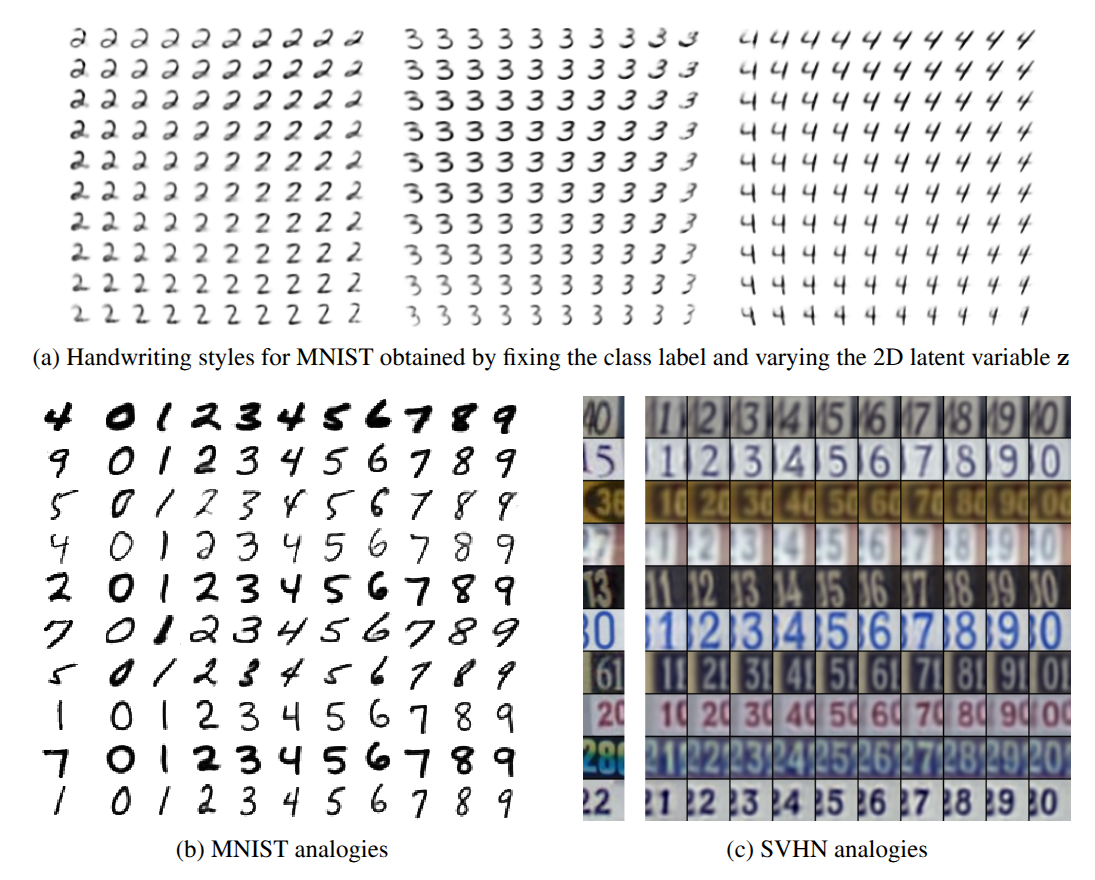
\includegraphics[height=0.7\textheight]{docs/slides/img/Screenshot from 2026-05-09 23-11-31.png}
\end{frame}

\begin{frame}
    \frametitle{\cite{gomez2018automatic}}
    \centering
    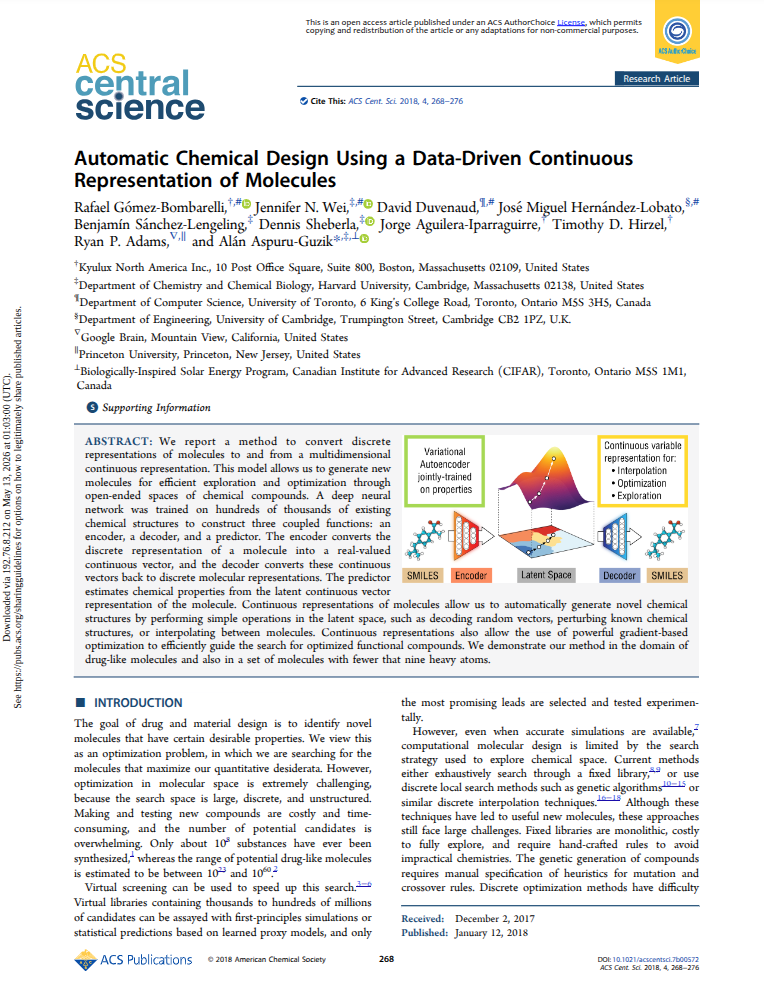
\includegraphics[height=0.8\textheight]{docs/slides/img/Auto chem design paper.png}
\end{frame}

\begin{frame}
    \frametitle{\cite{gomez2018automatic}}
    \begin{columns}
        \begin{column}{0.45\textwidth}
            \begin{itemize}
                \setlength{\itemsep}{2em}
                \item[$\bigstar$] Generate new molecules with desirable properties
                \item Train VAE on SMILES strings
                \item SMILES = ``Simplified Molecular Input Line Entry System''
                \item Chemical structure $\rightarrow$ ASCII string
            \end{itemize}
        \end{column}
        \hfill
        \begin{column}{0.45\textwidth}
            \centering
            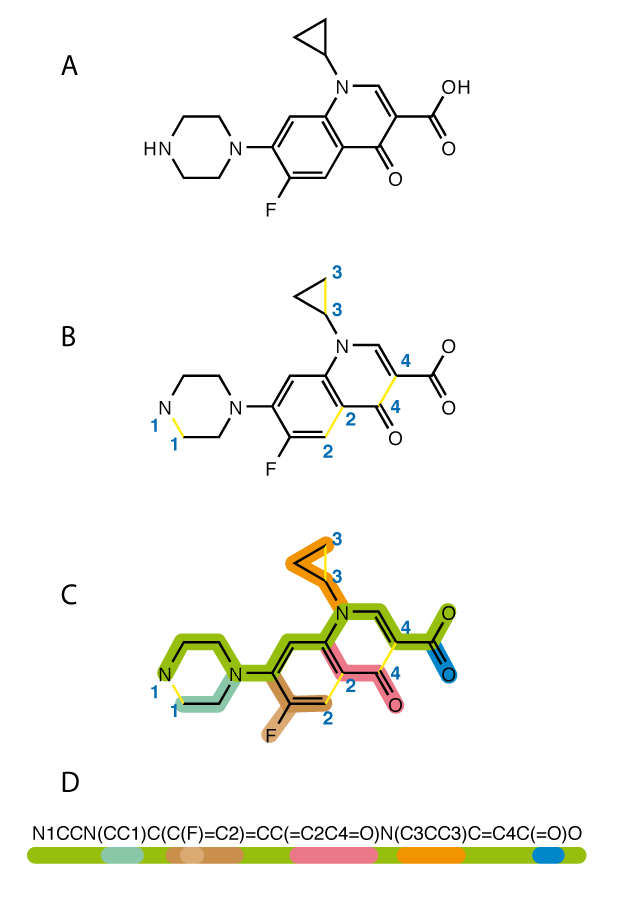
\includegraphics[height=0.8\textheight]{docs/slides/img/SMILES.png}
            \tiny \url{https://en.wikipedia.org/wiki/Simplified_Molecular_Input_Line_Entry_System}
        \end{column}
    \end{columns}
\end{frame}

\begin{frame}
    \frametitle{\cite{gomez2018automatic}}
    \begin{itemize}
        \setlength{\itemsep}{0.8em}
        \item Train $f_\text{enc}(x_\text{SMILES}) = z_n$
        \item Train $f_\text{dec}(z_n) = x_\text{SMILES}$
        \item $f_\text{enc}, f_\text{dec}$ = CNNs or RNNs
        \item Train $f_\text{prop}(z_n) = \pi$, $f_\text{prop}$ = MLP or GP, $\pi = \dots$
        \begin{itemize}
            \item ``logP'' = water-octanol partition coefficient
            \item ``SAS'' = synthetic accessibility score
            \item ``QED'' = Quantitative Estimation of Drug-likeness
            \item \dots
        \end{itemize}
        \item To sample molecules with properties $\pi^*$:
        \begin{itemize}
            \item $z_n = \text{argmin}_{z_n}\Bigl[ \mathcal{L}\Bigl(f_\text{prop}(z_n), \pi^*\Bigr) \Bigr]$ (EG SGD, BP through $f_\text{prop}$)
            \item $f_\text{dec}(z_n) = x_\text{SMILES}$
        \end{itemize}
    \end{itemize}
\end{frame}

\begin{frame}
    \frametitle{\cite{gomez2018automatic}}
    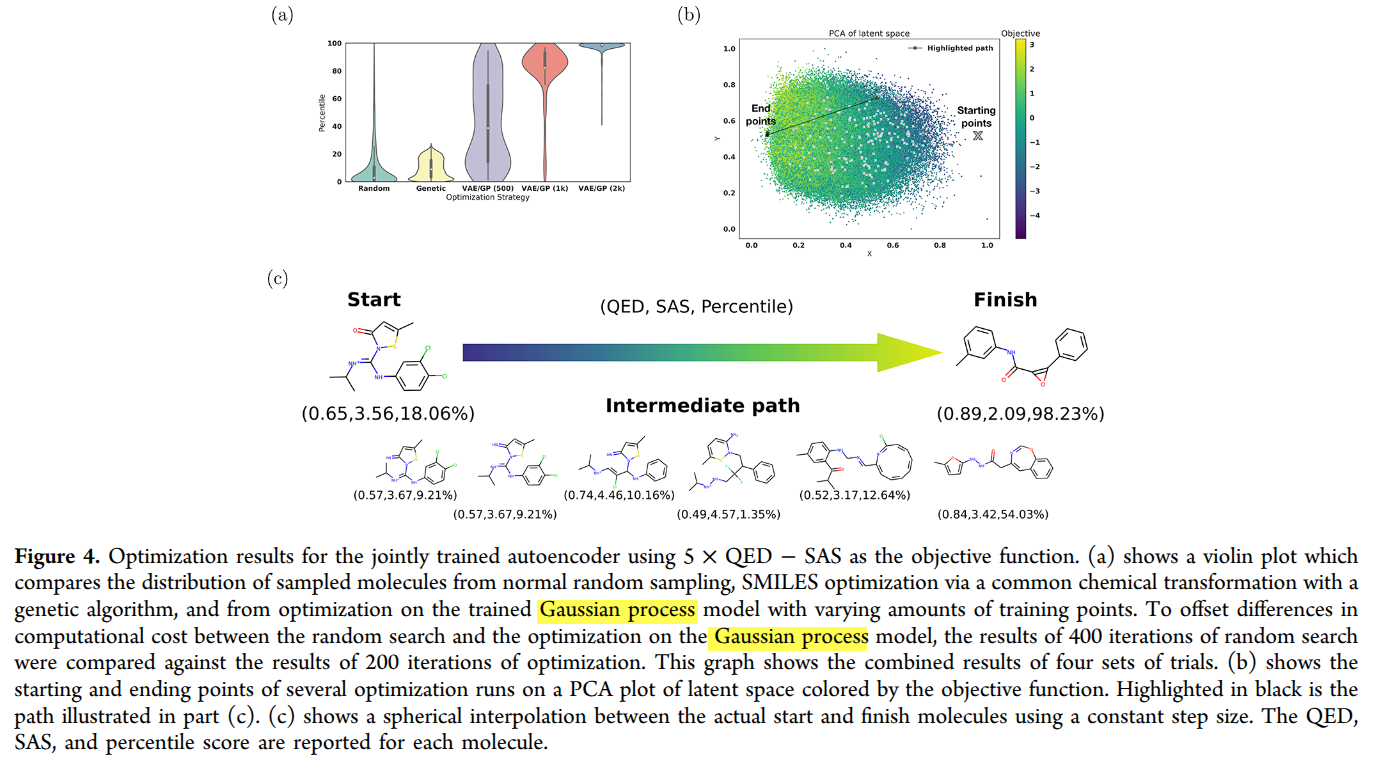
\includegraphics[width=\textwidth]{docs/slides/img/VAE GP molecule samples.png}
\end{frame}

\begin{frame}
    \frametitle{VAE molecule generation developments}
    \begin{itemize}
        \setlength{\itemsep}{1em}
        \item \sout{SMILES} Encode/decode molecular graphs directly \cite{jin2018junction}
        \item \emph{Constrained} BO $\Rightarrow$ avoid generating invalid molecules \cite{griffiths2020constrained}
        \item ``Deep metric learning'' EG $\mathcal{L}_\text{triplet}(x^b, x^+, x^-)$ $\Rightarrow$ improve VAE latent space structure $\Rightarrow$ improve BO performance \cite{grosnit2021high}
        \item Adapt trust regions to account for input space structure \cite{maus2022local}
        \item Using ``pretrained ProtT5nv transformer-based T5 encoder and decode'' in the VAE pipeline \cite{sevgen2025prot}
        \item \dots
    \end{itemize}
\end{frame}

\begin{frame}
    \frametitle{The end.}
    \centering
    \includegraphics{example-image-duck}
\end{frame}

\bibliographystyle{apalike}
\bibliography{../references}

\end{document}
